\subsection{Flujo de caja}

El flujo de caja permite hacer seguimiento del dinero de la empresa, teniendo como resultado la capacidad de poder pagar las deudas y gastos, de igual forma determinar la liquidez del negocio. En la tabla \ref{flujoCaja} se ilustra mejor.

\vspace{2mm}
\begin{minipage}{0.8\textwidth}
\centering
\captionof{table}[{Flujo de caja }]{ Flujo de caja }
\label{flujoCaja}
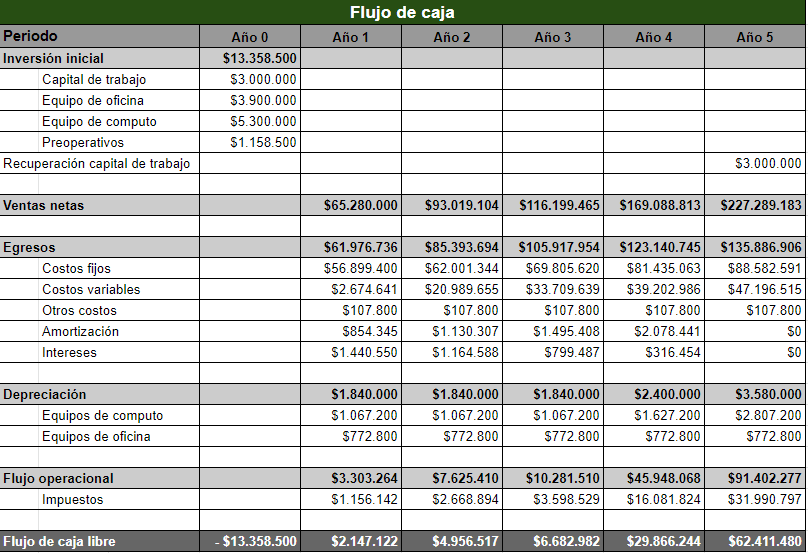
\includegraphics[width=1.2\textwidth]{Images/flujoCaja.png}
\fnote{Nota. \textup{Fuente : Autores}}
\end{minipage}
\newpage